%!TEX TS-program = xelatex
%!TEX encoding = UTF-8 Unicode
\documentclass[12pt,a4paper]{article}
\usepackage{geometry} % 設定邊界
\geometry{
  top=1in,
  inner=1in,
  outer=1in,
  bottom=1in,
  headheight=3ex,
  headsep=2ex
}
\usepackage{fontspec} % 允許設定字體
\usepackage{xeCJK} % 分開設置中英文字型
\usepackage{url} % 使用url
\usepackage[colorlinks,
            linkcolor= black]{hyperref}
\setCJKmainfont{LiHei Pro} % 設定中文字型
\setmainfont{Georgia} % 設定英文字型
\setromanfont{Georgia} % 字型
\setmonofont{Courier New}
\linespread{1.2}\selectfont % 行距
\XeTeXlinebreaklocale "zh" % 針對中文自動換行
\XeTeXlinebreakskip = 0pt plus 1pt % 字與字之間加入0pt至1pt的間距,確保左右對整齊
\parindent 0em % 段落縮進
\setlength{\parskip}{20pt} % 段落之間的距離

\title{\huge 物聯網應用與資料分析 Assignment3 - 構建一個有專家系統的IoT Web} % 設置標題,使用巨大字體
\author{姓名:吳嘉偉\quad 學號:5105056013\quad 日期:2018/4/28} % 設置作者
\date{} % 設置日期
\usepackage{titling}
\setlength{\droptitle}{-8em} % 將標題移動至頁面的上面
\usepackage{listings}

% 設置演算法的灰色底
\usepackage{algorithmic}
\usepackage{color}
\definecolor{algorbgm}{gray}{0.85}
\newcommand{\grayblock}[1]{
\colorbox{algorbgm}{\centering
\begin{minipage}{0.8\textwidth} ~\\[-15pt]#1~\\[-25pt] \end{minipage}}}
% example
%\begin{algorithmic}
%\IF{somebody open the door 1}
%\STATE he gets an apple
%\STATE he gets an key
%\ELSIF{somebody open the door 2}
%\STATE he gets nothing
%\ENDIF
%\end{algorithmic}

% 設置灰底
\usepackage{color}
\usepackage{framed}
\definecolor{shadecolor}{gray}{0.85}
% example
%\begin{shaded}
%java -jar test.jar	
%\end{shaded}

\begin{document}

\clearpage

\maketitle % 顯示標題

\section{目標}
{
\fontsize{14pt}{10pt} % 字型大小14pt,字行間距20pt
\selectfont % 生效
希望可以透過專家系統,把數值訓練成在某一數值以上或以下用不同的顏色區分,並把結果畫出曲線產生在網頁上。
\begin{figure}[ht]
\centering
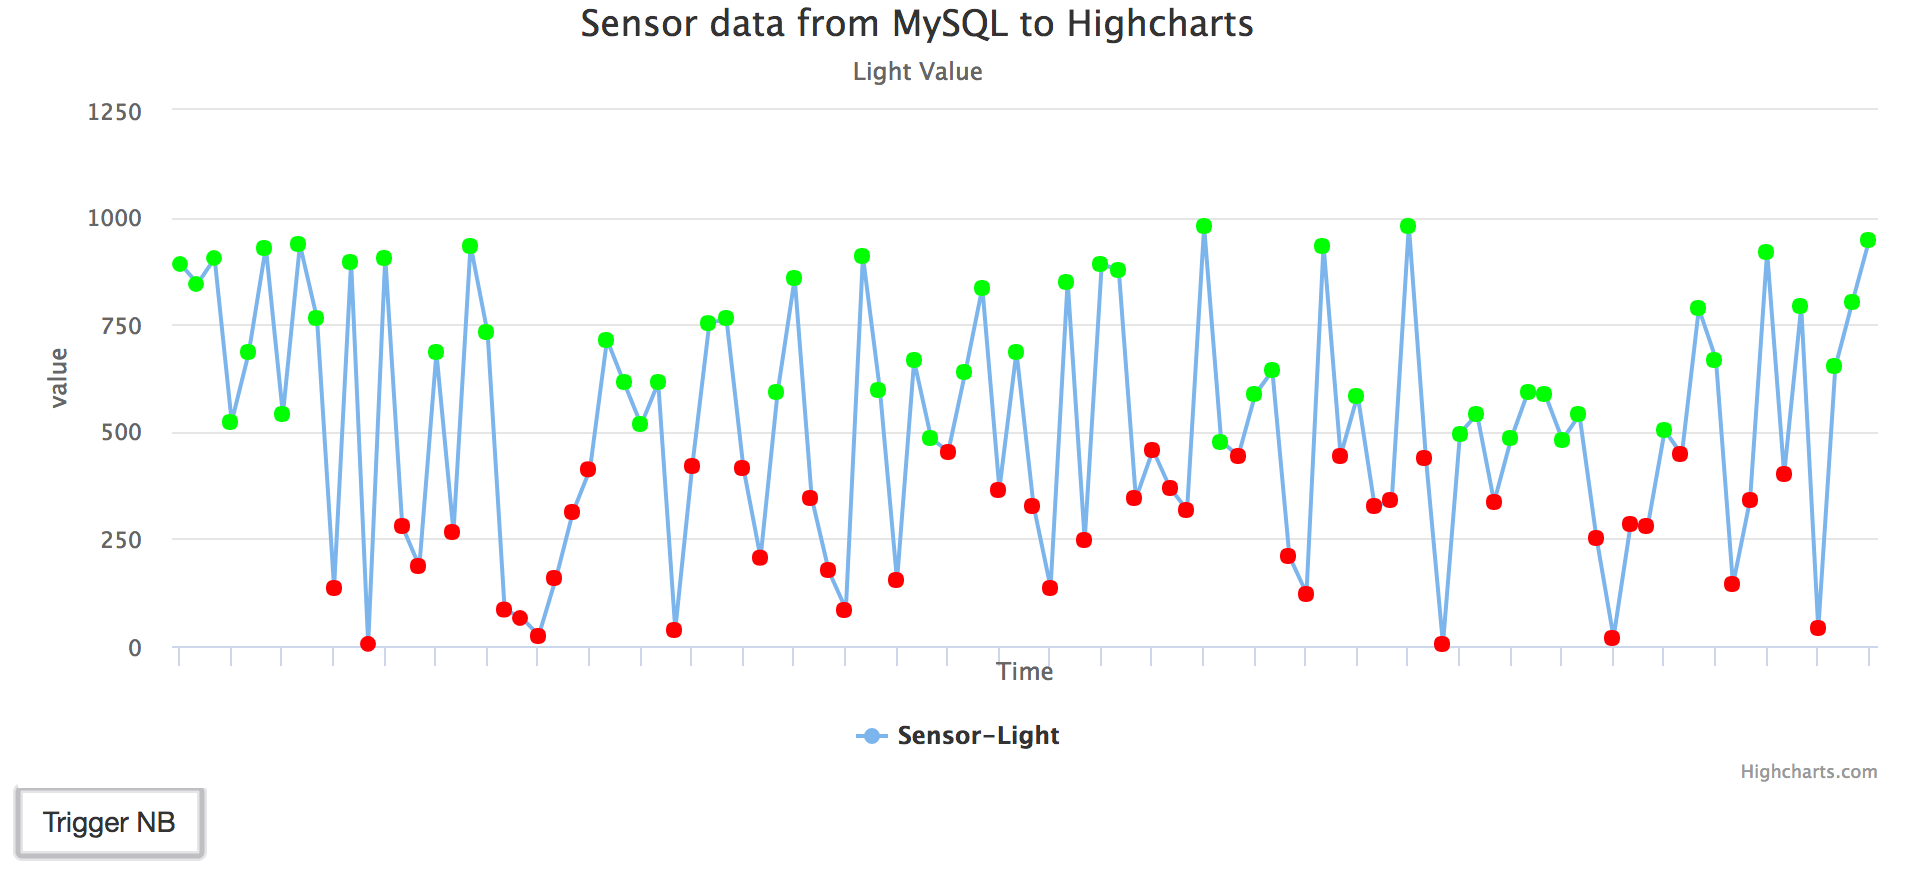
\includegraphics[width=1.0\textwidth]{image/resultcharts.png}
\end{figure}
}

\newpage % 新一頁
\section{產生資料庫資料}
{
\subsection{建立資料庫}
利用create.php建立一個新的資料庫

程式碼:
\begin{shaded}
\begin{lstlisting}[language=PHP]
<?php
/*
* 自動建立資料庫及資料表
* 欄位:
*       id      -> int (主鍵)
*       data    -> int
*       time    -> TIMESTAMP (CURRENT_TIMESTAMP)
*/
//IP、帳號資訊
$host = "172.32.16.42";
$user = "iot";
$pass = "iot";
//資料庫資訊
$databaseName = "lightdb";
$tableName = "light";
//連線資料庫伺服器
$con = mysqli_connect($host,$user,$pass);
//建立資料庫
$sql = "CREATE DATABASE $databaseName";
mysqli_query($con, $sql);
//連結資料庫
$dbs = mysqli_select_db($con, $databaseName);
//建立資料表
$sql = "CREATE TABLE ". 
   "`$tableName`( `id` INT NOT NULL AUTO_INCREMENT , ".           
   "`value` INT NOT NULL , ".
   "`status` INT NOT NULL , ".
   "`time` TIMESTAMP NOT NULL DEFAULT CURRENT_TIMESTAMP ,".        
   " PRIMARY KEY (`id`)) ENGINE = InnoDB";
mysqli_query($con, $sql);
?>
\end{lstlisting}
\end{shaded}

\subsection{產生隨機的數值與狀態}
利用dataset.php隨機得產生數值與狀態

程式碼:
\begin{shaded}
\begin{lstlisting}[language=PHP]
<?php

$host = "172.32.16.42";
$user = "iot";
$pass = "iot";

//資料庫資訊
$databaseName = "lightdb";
$tableName = "light";

//連結資料庫
$con = mysqli_connect($host,$user,$pass);
$dbs = mysqli_select_db($con, $databaseName);

for($i=0;$i<100;$i++) {
	$sql = "INSERT INTO $tableName (value,status) 
		VALUES (".rand(0,1023).",".rand(0,1).")";
	mysqli_query($con, $sql);
}

?>
\end{lstlisting}
\end{shaded}

\subsection{趨勢圖}
{
到目前為止,我們就可以產生一個狀態是隨機的趨勢圖
\begin{figure}[ht]
\centering
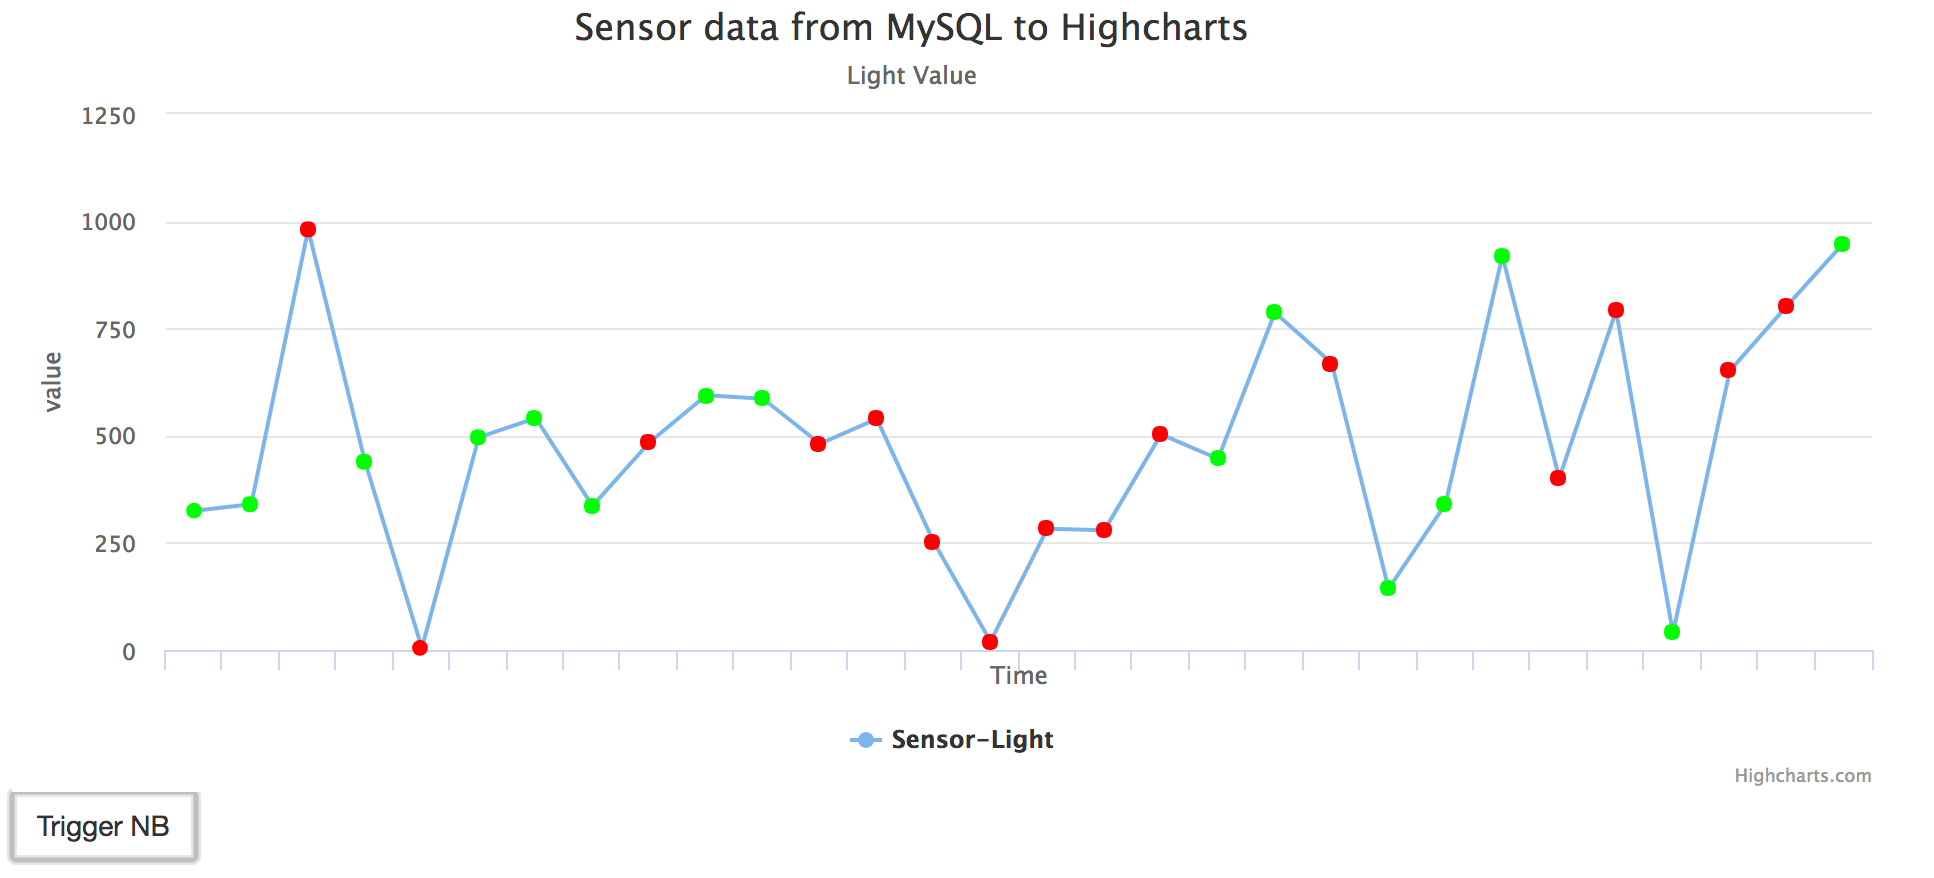
\includegraphics[width=1.0\textwidth]{image/defaultcharts.png}
\end{figure}
}

\newpage
\section{專家系統}
{
\subsection{產生訓練資料}
先用Excel產生一列隨機亂數,並在第二列寫上狀態,如果數值大於500為1,否則為0,
用此檔案當成訓練資料。

\begin{figure}[ht]
\centering
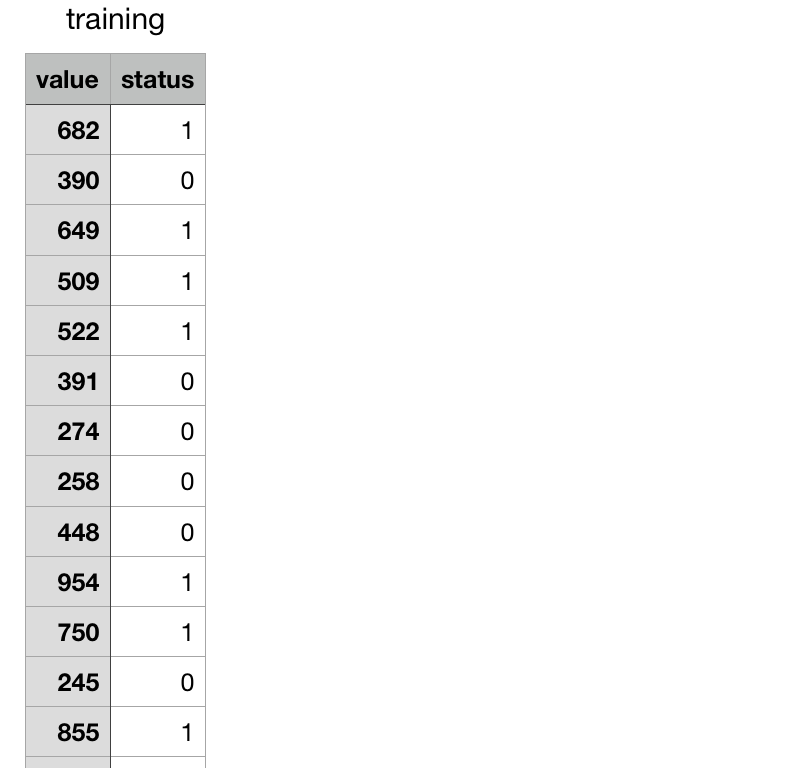
\includegraphics[width=1.0\textwidth]{image/trainingData.png}
\end{figure}

\newpage
\subsection{訓練資料}
利用Python的sklearn,把上一步驟產生的檔案用來訓練資料庫的資料並給予正確的狀態
\begin{shaded}
\begin{lstlisting}[language=Python]
# read training data
data = pandas.read_csv("training.csv")
pdX = data["value"]
npX = numpy.array(pdX)
npX = npX.reshape(-1, 1)

pdY = data["status"]
npY = numpy.array(pdY)

# sklearn
clf = lm.LogisticRegression()
clf.fit(npX, npY)
\end{lstlisting}
\end{shaded}

\subsection{訓練資料庫數值}
利用剛剛產生的LogisticRegression來訓練資料庫的資料,並把訓練完的結果寫入資料庫
\begin{shaded}
\begin{lstlisting}[language=Python]
# connect db
db = pymysql.connect("172.32.19.7", "iot", "iot", "lightdb")
cursor = db.cursor()

# 執行SQL語法查詢
cursor.execute("SELECT * FROM light")

# 整理搜尋出來的資料
id_list = []
value_list = []
results = cursor.fetchall()
for row in results:
  id_list.append(row[0])
  value_list.append(row[1])

# 把結果轉為ndarray
predictValues = numpy.array(value_list)
predictValues = predictValues.reshape(-1, 1)

# 把values丟到LogisticRegression預測狀態
predictStatus = clf.predict(predictValues)
status_list = predictStatus.tolist()

# 更新資料庫狀態
for i in range(len(id_list)):
  id = id_list[i]
  status = status_list[i]
  cursor.execute("update light set status = %d 
  	where id = %d" % (status, id))
  db.commit()

# 關閉資料庫
db.close()
\end{lstlisting}
\end{shaded}

\subsection{輸出結果}
把訓練後的資料組成json格式後輸出回去

\begin{shaded}
\begin{lstlisting}[language=Python]
# 輸出結果
result = json.dumps([{'value': rowValue, 'status': status} 
	for rowValue, status in zip(value_list, status_list)])
print(result)
\end{lstlisting}
\end{shaded}

\section{HighChart}
\subsection{新增按鈕}
在趨勢圖的下方新增一個按鈕,用來觸發訓練事件

\begin{shaded}
\begin{lstlisting}[language=Html]
<div class="container">
	<div id="container" 
		style="min-width: 310px; 
		height: 400px; 
		margin: 0 
		auto">Insert Highchart Here</div>
	<button class = "btn byn-info" 
			id = "trigger">Trigger NB</button>
</div>
\end{lstlisting}
\end{shaded}

\begin{shaded}
\begin{lstlisting}[language=Html]
$('#trigger').click(function(){
	$.ajax({
		url: 'triggerNB.php',//連接的URL	 
		data: "{}",//夾帶的參數
		dataType: 'json', //資料格式
		success: function(data)	//傳送成功的function
		{
			alert("success");
		},
		error: function(XMLHttpRequest, 
			textStatus, errorThrown) {
            alert("Error: " + errorThrown); 
        }
	});
});
\end{lstlisting}
\end{shaded}

\subsection{Php呼叫python}
利用excu(),呼叫python,並把結果輸出給highchart

\begin{shaded}
\begin{lstlisting}[language=Php]
<?php

	$output = exec('/Library/Frameworks/Python.framework
	/Versions/3.6/bin/python3.6 ./linear_model.py');
	echo ($output);
?>
\end{lstlisting}
\end{shaded}

\subsection{解析回傳資料}
把php吐回來的資料解析後重新畫趨勢圖

\begin{shaded}
\begin{lstlisting}[language=Html]
values = [];
time = [];
for (var i = 0; i < data.length; i++)
{
	if(parseInt(data[i]['status']) == 0)
		values.push({y:parseInt(data[i]['value']), 
			color: '#FF0000' });
	else
		values.push({y:parseInt(data[i]['value']), 
			color: '#00FF00' });
	time.push(data[i]['time']);
}
highcharsinit();
\end{lstlisting}
\end{shaded}

\newpage
\subsection{執行結果}
訓練後的結果,當value = 480左右做個區隔
\begin{figure}[ht]
\centering
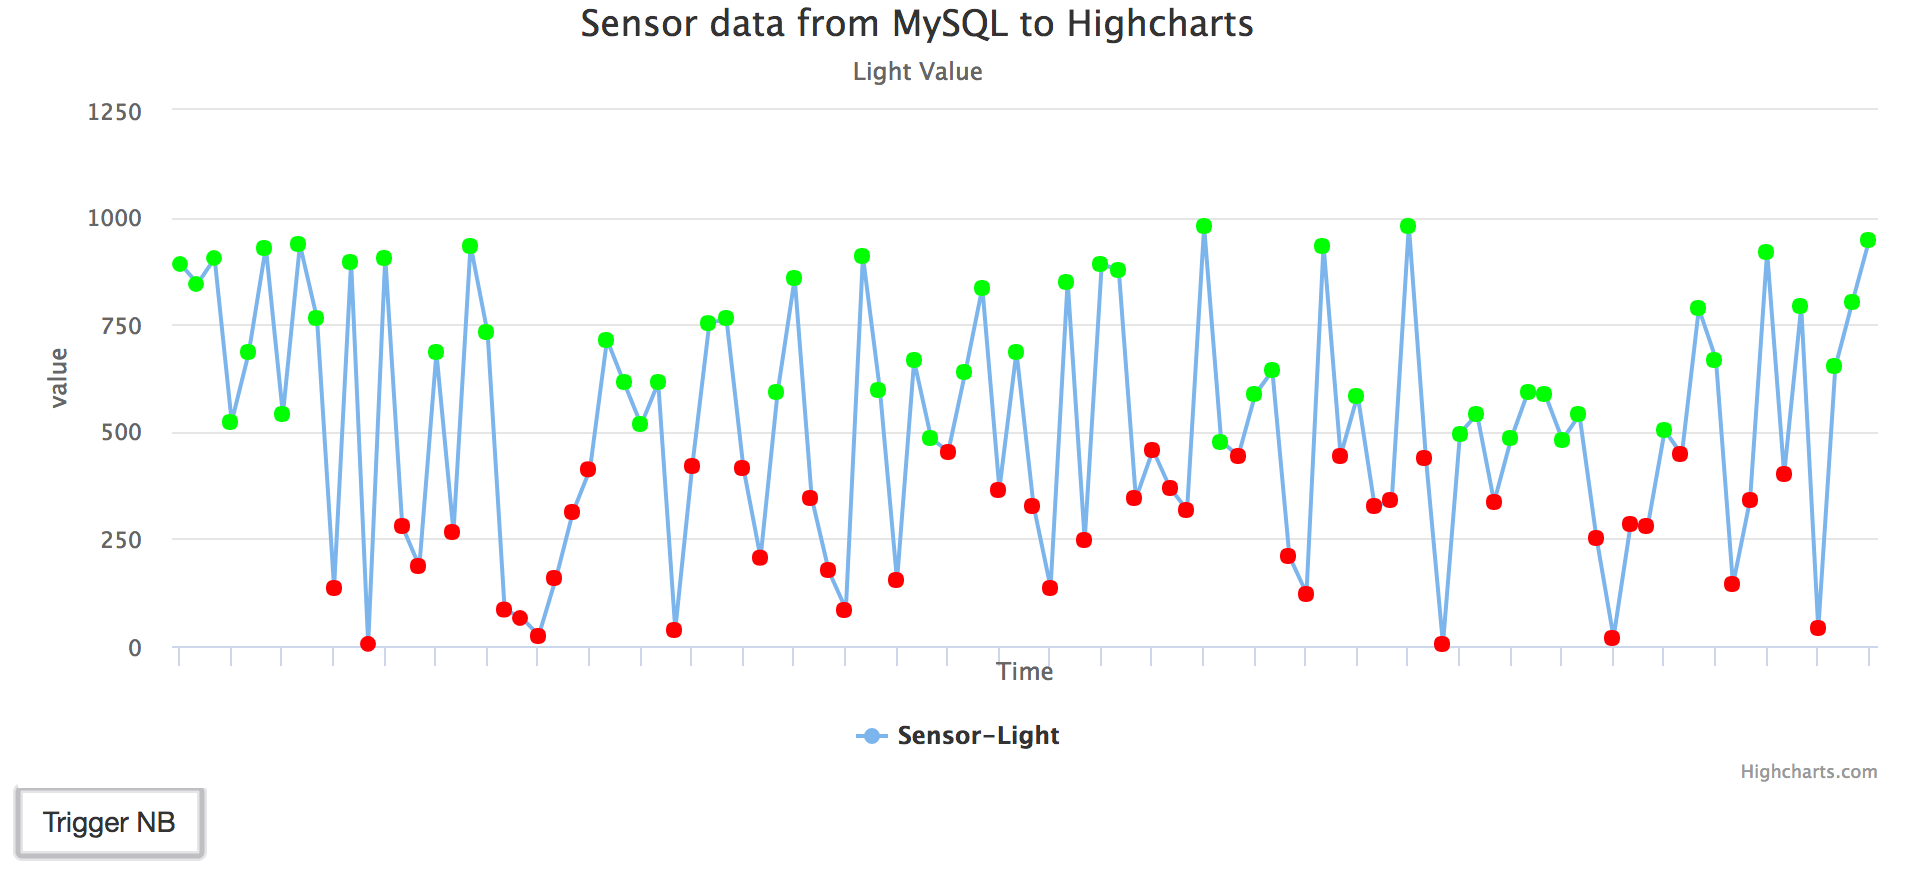
\includegraphics[width=1.0\textwidth]{image/resultcharts.png}
\end{figure}

\end{document}